\section{Enforcing a contract by accounting}
\label{sec:method}

This section develops the mechanism. Section~\ref{sec:gate} states the
ledger gate and proves that it makes the contract unbreakable;
Section~\ref{sec:feasible} characterises what becomes attainable once
declining is an action; Section~\ref{sec:optimise} gives the
optimisation layer and its regret; Section~\ref{sec:labels} prices
partial labelling; Section~\ref{sec:width} compares the concession this
design makes with the one a calibration certificate makes.

\begin{figure*}[t]
\centering
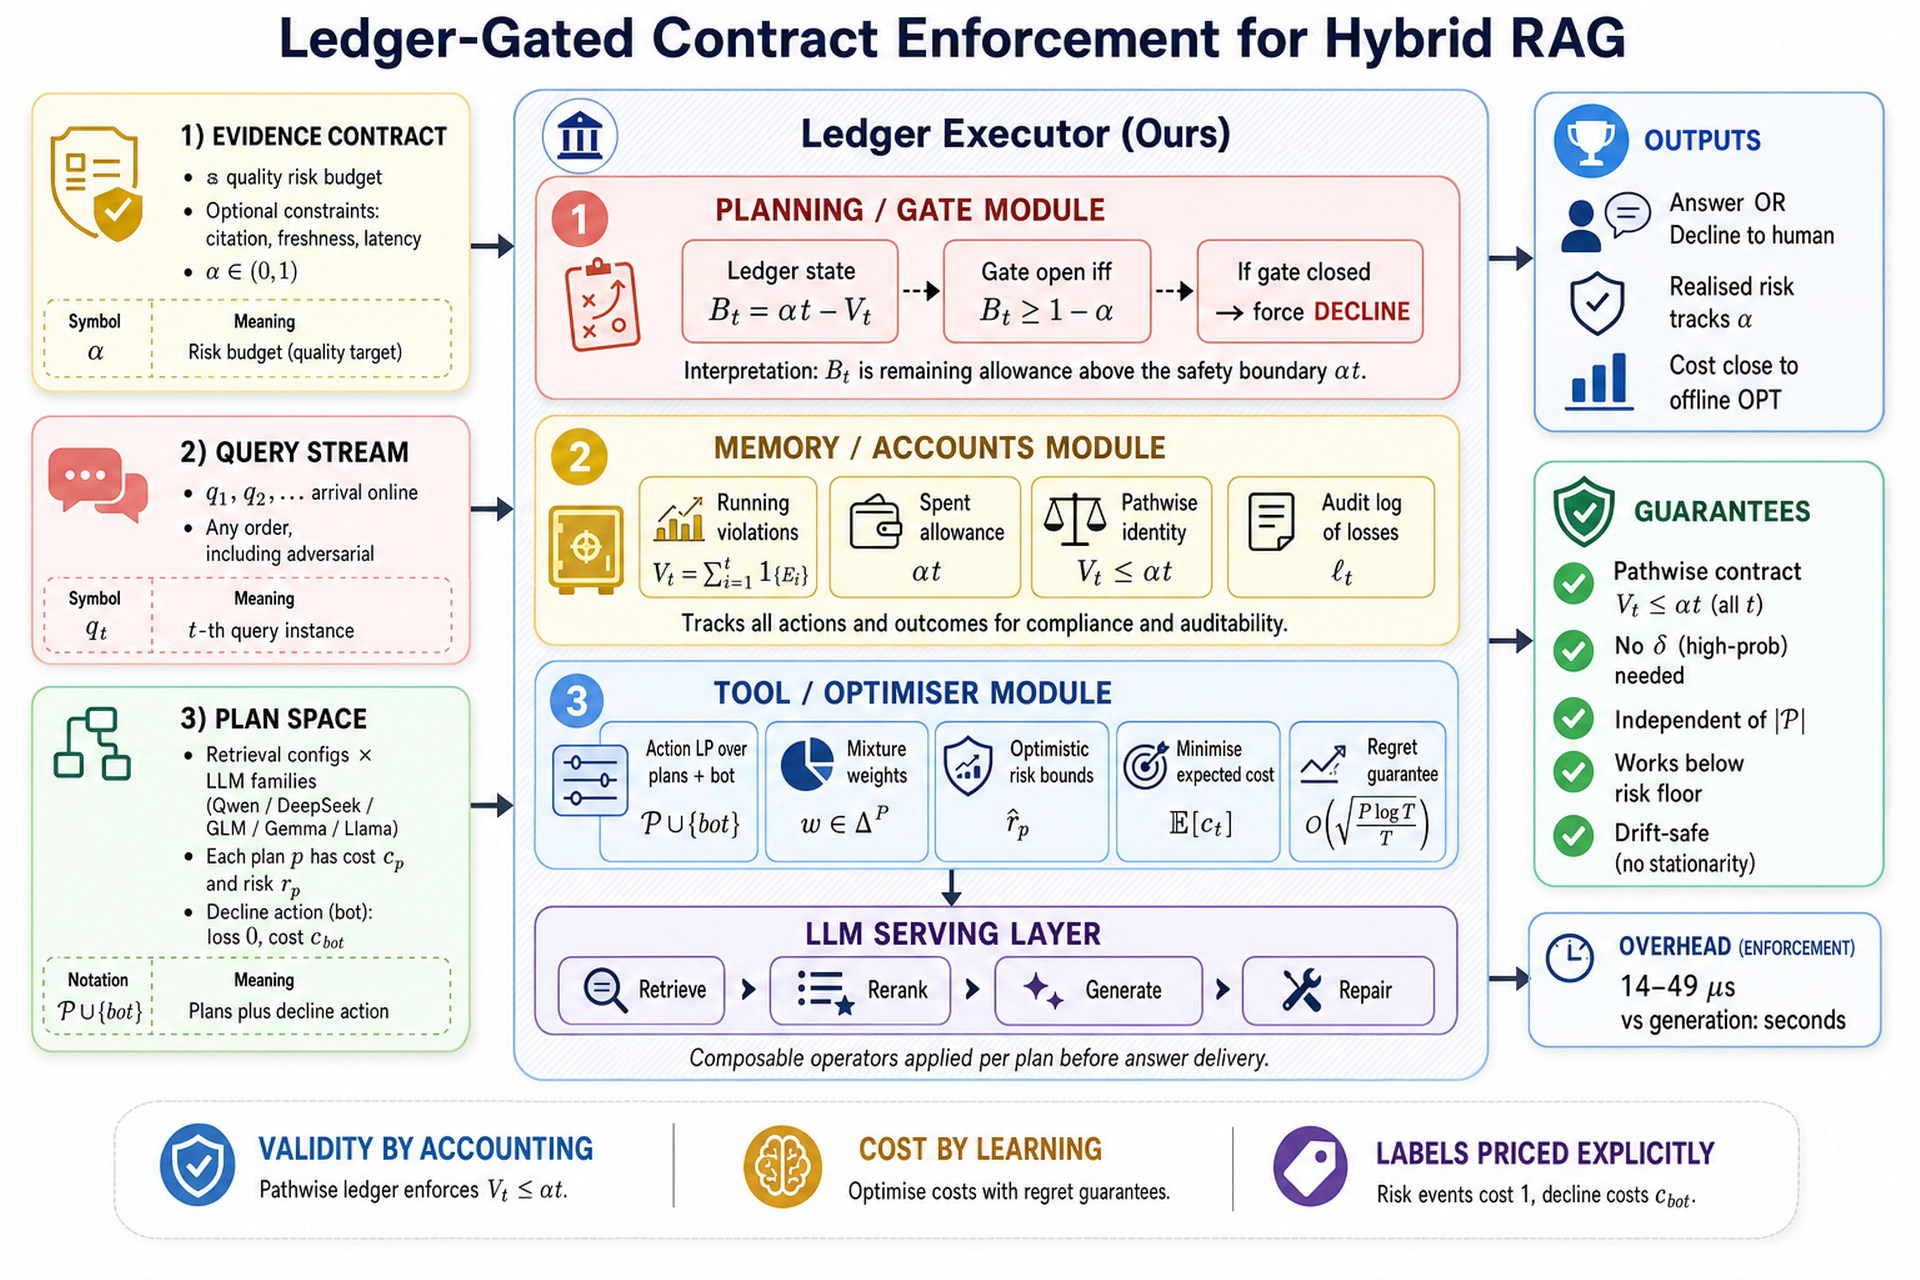
\includegraphics[width=\textwidth]{figures/fig_method_ledger}
\caption{System overview of ledger-gated contract enforcement.
Left: the evidence contract, the online query stream (any order) and
the hybrid RAG plan space including the decline action $\bot$.
Centre: the executor separates a gate that enforces
$B_t=\alpha t-V_t$, an account of realised losses, and an action LP
that minimises cost under optimistic risk estimates; the LLM serving
layer is unchanged.
Right: answers or declines, with pathwise guarantees independent of
$\delta$ and $|\mathcal{P}|$, at microsecond enforcement cost.}
\label{fig:method}
\end{figure*}

\begin{figure*}[t]
\centering
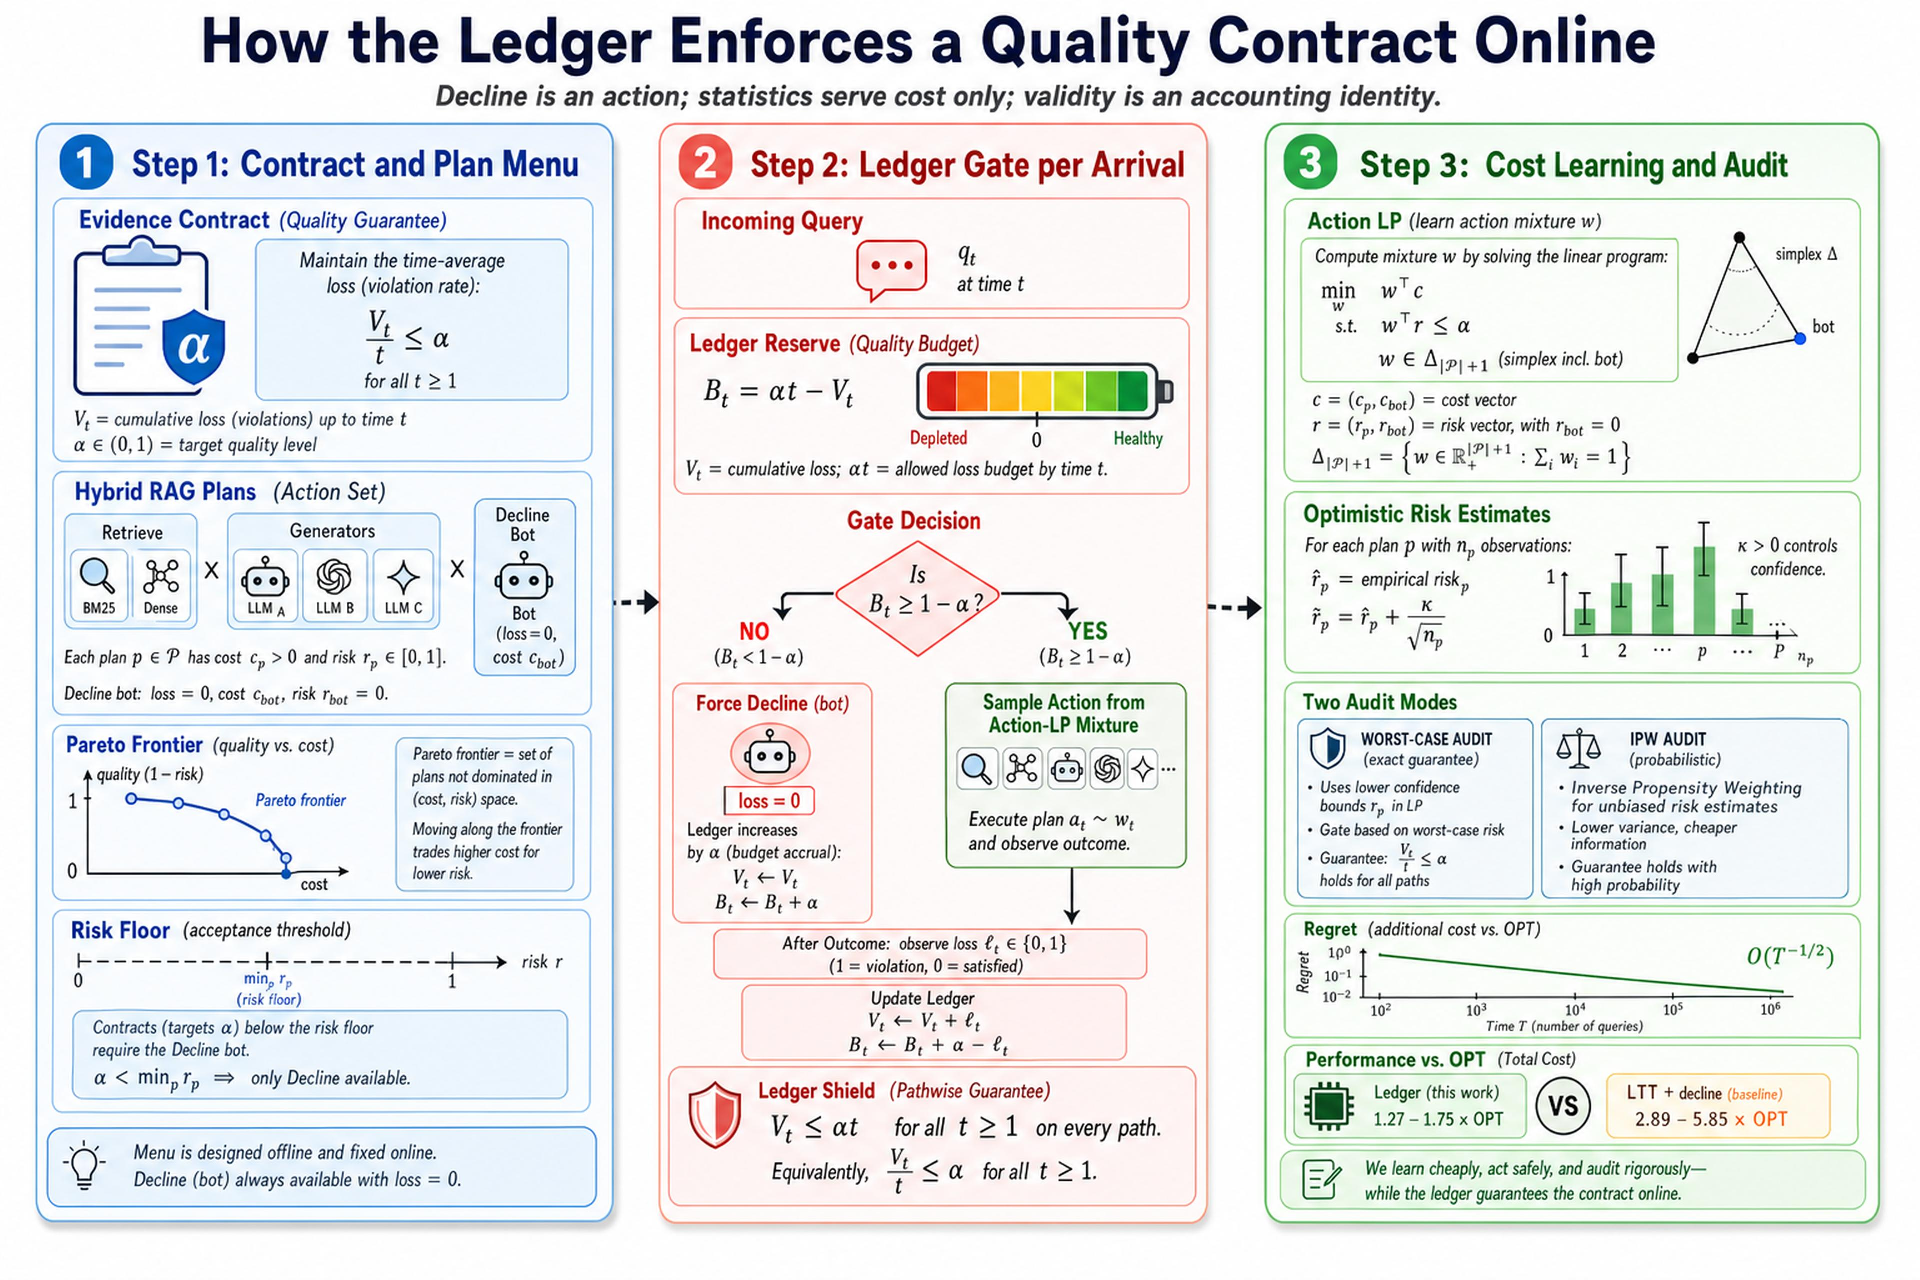
\includegraphics[width=\textwidth]{figures/fig_pipeline_ledger}
\caption{Online operation in three stages.
(1)~A fixed plan menu plus $\bot$ makes every $\alpha>0$ attainable,
including levels below the risk floor $\min_p r_p$.
(2)~At each arrival the gate tests $B_{t-1}\ge 1-\alpha$; a closed
gate forces decline, an open gate samples from the action mixture, and
the ledger is updated from the observed loss so that
$V_t\le\alpha t$ holds on every path.
(3)~Cost is learned by an optimistic LP over plans plus declining, with
worst-case or inverse-probability auditing; regret decays as
$O(T^{-1/2})$ and the bill stays at $1.27$--$1.75\times$ the offline
optimum where the same-action-space certifier pays
$2.89$--$5.85\times$.}
\label{fig:pipeline}
\end{figure*}

\subsection{The ledger gate}
\label{sec:gate}

Fix a contract level $\alpha \in (0,1)$ and write $\ell_t \in [0,1]$ for
the violation loss incurred on the $t$-th arrival. Define the
\emph{ledger}
\begin{equation}
\label{eq:ledger}
B_t \;=\; \alpha t - V_t ,
\qquad V_t \;=\; \sum_{s\le t} \ell_s ,
\qquad B_0 = 0 ,
\end{equation}
the contract allowance earned but not yet spent. The controller is the
following rule, and nothing else is needed for validity.

\begin{definition}[Ledger gate]
\label{def:gate}
At arrival $t$ the executor may run any plan $p \in \mathcal{P}$ if
$B_{t-1} \ge 1 - \alpha$; otherwise it must take the decline action
$\bot$, for which $\ell_t = 0$ by definition.
\end{definition}

\begin{theorem}[Pathwise contract satisfaction]
\label{thm:gate}
Under Definition~\ref{def:gate}, $B_t \ge 0$ and hence
\begin{equation}
\label{eq:pathwise}
V_t \;\le\; \alpha t
\qquad\text{for every } t \ge 1 ,
\end{equation}
on every sample path, for every query sequence, whatever plan the
executor chooses when the gate is open.
\end{theorem}

\begin{pf}
Induction on $t$. $B_0 = 0 \ge 0$. Suppose $B_{t-1}\ge 0$. If the gate
is open then $B_{t-1} \ge 1-\alpha$, and since $\ell_t \le 1$,
\[
B_t = B_{t-1} + \alpha - \ell_t \;\ge\; (1-\alpha) + \alpha - 1 = 0 .
\]
If the gate is closed the executor declines, $\ell_t = 0$, and
$B_t = B_{t-1} + \alpha \ge B_{t-1} \ge 0$. In both cases
$B_t \ge 0$, which is~\eqref{eq:pathwise}.
\end{pf}

Three things are absent from this argument and their absence is the
contribution. There is no probability: \eqref{eq:pathwise} is not an
event of probability $1-\delta$ but an identity of the realised
trajectory. There is no distributional assumption: the queries may be
adversarial, adaptively chosen against the executor, or drawn from a
distribution that changes at every step, and the bound is unaffected --
so drift needs no detector, no restart schedule and no error budget,
because there is no assumption for drift to falsify. And there is no
dependence on $|\mathcal{P}|$: the executor may consider a hundred
plans or a million, and pays nothing for having considered them, which
is exactly the multiplicity price a calibration certificate cannot
avoid.

What Theorem~\ref{thm:gate} does not do is make the system useful. It
would be satisfied by declining every query. The content of the design
is that validity has been removed from the optimisation problem
entirely, so the optimiser can be judged on cost alone -- and, being
unable to cause a violation, can be far more aggressive than a
certifier is allowed to be. The rest of this section is about cost.

\begin{rmk}[Bounded losses]
The gate uses $\ell_t \le 1$ to size the reserve $1-\alpha$. For a
bounded loss $\ell_t \le L$ the same argument gives the gate
$B_{t-1}\ge L-\alpha$; for an unbounded loss no deterministic reserve
exists and the guarantee necessarily becomes probabilistic. Contract
losses in this setting are indicators of an audit predicate
(Section~\ref{sec:prelim}) and are bounded by construction.
\end{rmk}

\subsection{What declining makes attainable}
\label{sec:feasible}

Let $r_p = \E[\ell(p,q)]$ and $c_p = \E[c(p,q)]$ be the risk and cost of
plan $p$ under the query distribution, and let the decline action have
risk $0$ and cost $c_\bot$. A randomised policy is a distribution $w$
over $\mathcal{P}\cup\{\bot\}$, and the offline problem is the linear
program
\begin{equation}
\label{eq:alp}
\mathrm{OPT}(\alpha) \;=\;
\min_{w \in \Delta} \; \sum_a w_a c_a
\quad\text{s.t.}\quad \sum_a w_a r_a \;\le\; \alpha .
\end{equation}

\begin{proposition}[Feasibility and its price]
\label{prop:feasible}
Without the decline action, \eqref{eq:alp} is feasible if and only if
$\alpha \ge \min_p r_p$. With it, \eqref{eq:alp} is feasible for every
$\alpha > 0$, and if $\alpha < \min_p r_p$ every feasible policy
declines at least a fraction $1 - \alpha/\min_p r_p$ of arrivals.
Moreover an optimal solution of \eqref{eq:alp} has at most two nonzero
weights.
\end{proposition}

\begin{pf}
The attainable risks of the plan-only simplex form the interval
$[\min_p r_p, \max_p r_p]$, giving the first claim. Declining
everything has risk $0$, so the feasible set is nonempty for any
$\alpha>0$. If $\sum_a w_a r_a \le \alpha$ and $r_a \ge \min_p r_p$ for
every $a \ne \bot$, then $(1-w_\bot)\min_p r_p \le \alpha$, i.e.\
$w_\bot \ge 1 - \alpha/\min_p r_p$. The last claim is the standard
basic-solution bound: \eqref{eq:alp} has two constraints, so a vertex
has at most two nonzero coordinates.
\end{pf}

Proposition~\ref{prop:feasible} is why declining cannot be dismissed as
a degenerate escape. Below $\min_p r_p$ the contract is unattainable by
any pipeline no matter how much is spent, so an optimizer that must
answer every query has nothing to return; the honest response is to
report how much traffic has to be routed elsewhere, and at what price.
This is the regime in which strict contracts live -- $\min_p r_p$ is
$0.59$ on two of our four tasks -- and it is invisible to the existing
formulation. The two-nonzero-weight property matters
operationally: the deployed policy is always "run plan $i$, or decline,
with probability $w$", never an opaque dense mixture.

\subsection{The optimisation layer and its regret}
\label{sec:optimise}

The risks $r_a$ are unknown, so the executor maintains an empirical mean
$\hat r_a$ over the labelled arrivals it has served with $a$, a count
$n_a$, and the mean observed cost $\hat c_a$. Costs and risks are
observed on different schedules and conflating them is a modelling
error: the price of a call is on the invoice when the call returns, so
$\hat c_a$ advances on every execution, whereas whether the answer was
acceptable requires an auditor and $\hat r_a$ advances only on labelled
ones. Every $\texttt{resolve\_every}$ arrivals the executor solves
\eqref{eq:alp} with $r_a$ replaced by
\begin{equation}
\label{eq:ucb}
\tilde r_a \;=\; \hat r_a + \kappa \sqrt{1/(4 n_a)}
\end{equation}
and samples its action from the optimal $w$. Algorithm~\ref{alg:ledger}
is the whole controller.

\begin{algorithm}[t]
\caption{Ledger-gated execution}
\label{alg:ledger}
\begin{algorithmic}[1]
\STATE $B \leftarrow 0$; $\hat r,\hat c$ from history; $n \leftarrow n_0$
\FOR{each arriving query $q_t$}
  \IF{$B \ge 1-\alpha$}
     \STATE $w \leftarrow$ solve \eqref{eq:alp} with $\tilde r$ from
            \eqref{eq:ucb} \quad(refreshed periodically)
     \STATE draw action $a \sim w$
  \ELSE
     \STATE $a \leftarrow \bot$ \quad\COMMENT{gate closed}
  \ENDIF
  \STATE execute $a$; pay $c_a$; observe loss $\ell_t$ if audited
  \STATE $B \leftarrow B + \alpha - \ell_t$
  \STATE update $\hat c_a$ always, $\hat r_a$ if audited
\ENDFOR
\end{algorithmic}
\end{algorithm}

The margin $\kappa/\sqrt{4n_a}$ in~\eqref{eq:ucb} deserves comment
because it resembles the object this paper argues against. Aiming the
mixture exactly at $\alpha$ is a mistake the ledger makes visible:
estimation error is two-sided, so a policy placed on $\alpha$ sits above
it half the time, the ledger drifts down, the gate closes and the
arrival is declined -- at $c_\bot$, the most expensive outcome
available. Steering slightly below $\alpha$ gives the ledger positive
drift and the gate stops firing. The margin is therefore a
cost-versus-cost device, and it differs from a confidence width in the
two ways that matter: it carries no part of the guarantee, so $\kappa$
is an $O(1)$ constant rather than $\sqrt{\log(K/\delta)}$ over a
candidate set, and its denominator is the number of arrivals served so
far, which grows without bound, so it decays to zero over the
deployment. Section~\ref{sec:width} quantifies both differences on our
data, and the experiments sweep $\kappa$ over $[0,4]$: cost moves by
$6$--$112\%$ across the sweep while the breach count stays at zero
throughout, which is what "the constant trades cost against cost" means
operationally.

\begin{theorem}[Cost regret]
\label{thm:regret}
Assume the stream is i.i.d.\ with plan risks $r_a$ and costs bounded by
$c_{\max}$, and let $\bar c_T$ be the mean serving cost of
Algorithm~\ref{alg:ledger} over $T$ arrivals. Then
\begin{equation}
\label{eq:regret}
\E[\bar c_T] - \mathrm{OPT}(\alpha)
\;=\; O\!\left( c_{\max} \sqrt{\frac{P \log T}{T}} \right) ,
\end{equation}
where $P = |\mathcal{P}|$.
\end{theorem}

\begin{pfsketch}
The proof has two parts.

\emph{Estimation.} Set $\kappa = \Theta(\sqrt{\log T})$. The
bounds $\tilde r_a$ dominate every $r_a$ at every $t \le T$ with
probability $1-O(T^{-1})$, by Hoeffding and a union bound over $P$ plans
and $T$ steps; on that event the LP solved by the executor is a
restriction of~\eqref{eq:alp}, so its value exceeds
$\mathrm{OPT}(\alpha)$ by at most the sensitivity of the LP to
tightening the constraint by $\max_a \kappa/\sqrt{4n_a}$. The value
function of~\eqref{eq:alp} is piecewise linear and convex in $\alpha$
with slope bounded by $c_{\max}/\min_{a\ne\bot} r_a$, giving a per-step
excess $O(c_{\max}\kappa/\sqrt{n_{a_t}})$. Summing over $t$ and using
$\sum_t n_{a_t}^{-1/2} = O(\sqrt{PT})$ yields the stated rate.
\emph{Gate closures.} While the estimates are accurate the deployed
mixture has risk at most $\alpha - \Omega(\kappa/\sqrt{n})$, so $B_t$ is
a random walk with positive drift; the expected number of arrivals at
which it is below the reserve $1-\alpha$ is $O(\sqrt{T})$ by the
reflection principle, each costing at most $c_{\max}$. Both terms are
$O(c_{\max}\sqrt{PT\log T})$ in total.
\end{pfsketch}

Note what Theorem~\ref{thm:regret} is and is not. It is an efficiency
statement and it does assume an i.i.d.\ stream; if that assumption
fails the cost degrades and the experiments in
Section~\ref{sec:results} measure by how much under four
non-exchangeable orderings. Theorem~\ref{thm:gate} keeps holding
throughout. Separating the two -- assumptions for efficiency,
none for safety -- is the structural difference from a calibration
certificate, where the same exchangeability assumption carries both.

\subsection{Paying for labels}
\label{sec:labels}

Theorem~\ref{thm:gate} consumes $\ell_t$ for every served query, which
in production means an auditor -- an LLM judge, or a human on sampled
traffic. Suppose only a fraction $\rho$ of served arrivals is labelled.
Two accounting rules are available and they differ in kind.

\begin{proposition}[Partial labelling]
\label{prop:labels}
If unlabelled arrivals are charged $\ell_t = 1$ (\emph{worst-case}
accounting), \eqref{eq:pathwise} continues to hold pathwise. If instead
they are charged $0$ and labelled ones are charged $\ell_t/\rho$
(\emph{inverse-probability} accounting), the ledger is an unbiased
estimate of $\alpha t - V_t$ and $V_t \le \alpha t + O(\sqrt{t\log(1/\delta)/\rho})$
holds with probability $1-\delta$ by Ville's inequality, but
\eqref{eq:pathwise} does not hold pathwise.
\end{proposition}

The first rule keeps a guarantee and pays for it in declines: an
unlabelled query consumes allowance as though it had failed, so the gate
closes sooner. The second keeps the cost and gives up the guarantee. We
report both, and the measured gap is not academic -- at $\rho = 0.25$,
worst-case accounting never breaches while inverse-probability
accounting breaches on $6\%$ (ASQA) to $59\%$ (HybridQA) of streams,
at essentially the same cost (Section~\ref{sec:results}). Auditing is
not free and this paper does not pretend otherwise; the audit bill is
carried in every cost figure we report, and on the cheapest contracts it
is the dominant term.

\subsection{Two concessions compared}
\label{sec:width}

Both designs give up something to be safe. A fixed-sequence certifier
concedes a confidence half-width
$w_{\mathrm{stat}} = \sqrt{\log(2K/\delta)/(2n_{\mathrm{cal}})}$: it
deploys a policy whose estimated risk is at most $\alpha -
w_{\mathrm{stat}}$, and since the decision is never revisited, that
slack is paid on every query for the life of the deployment. The ledger
concedes the reserve $1-\alpha$ and the margin
$\kappa/\sqrt{4n_a(t)}$. The reserve is a constant, so its per-query
cost $ (1-\alpha)/t $ vanishes; the margin shrinks as the deployment
serves traffic.

The gap is large on real numbers. With $K = 69$ candidates,
$\delta = 0.1$ and $n_{\mathrm{cal}} = 500$, $w_{\mathrm{stat}} =
0.085$; the ledger's margin after a stream of $6\,466$ HybridQA queries
concentrated on two or three plans is $\kappa/\sqrt{4n} = 0.011$ at
$\kappa=1$ -- $7.9\times$ tighter, and $2.8$--$4.4\times$ tighter on the
shorter streams -- and $0$ at $\kappa=0$, where validity is unchanged.
On a contract at $\alpha = 0.20$ the certifier is therefore steering at
$0.115$ while the ledger steers at $0.189$. It is not that the certifier
is insufficiently clever; it is aiming at a different and much stricter
target, and buying the plans that hit it. Table~\ref{tab:main} shows the
consequence directly: the certified policies realise risks far below the
contract they were given, which is wasted allowance paid for in
expensive plans and unnecessary declines.
